\section{Methodology}
\label{sec:method}

Fig.~\ref{fig:approach} lays out the study in eight stages: the data were audited and
windowed and the expected signal checked (stages 1--4), the evaluation framework and the plan
were fixed (stage 5), and only then were the questions answered (stages 6--8). This section
covers the data, tasks, hypotheses and statistics; Section~\ref{sec:arch} the decoders and
the software.

\begin{figure}[!t]
  \centering
  \scalebox{0.84}{% The approach in eight numbered stages (Chapter 3 opening). Colours as paper/figures/tikz/style.tex.
\begin{tikzpicture}[node distance=6mm and 5mm,
  stage/.style={draw, rounded corners=3pt, align=center, text width=27mm, minimum height=13mm,
    font=\footnotesize, line width=0.7pt},
  databox/.style={stage, draw=rblue, fill=rblue!8},
  studybox/.style={stage, draw=black!70, fill=white},
  explorebox/.style={stage, draw=black!55, dashed, fill=white},
  outbox/.style={stage, draw=rorange, fill=rorange!12},
  flow/.style={-{Stealth[length=2mm]}, line width=0.7pt, draw=black!75},
  num/.style={circle, draw=black!70, fill=white, inner sep=0.8pt, font=\scriptsize\bfseries}]
  \node[databox] (s1) {Public recording\\ \nSubjects{} stroke patients};
  \node[databox, right=of s1] (s2) {Integrity audit\\ duplicates, events};
  \node[databox, right=of s2] (s3) {4-second pieces\\ rest, hand, sixth finger};
  \node[databox, right=of s3] (s4) {Signal check\\ the mu rhythm falls};
  \node[stage, draw=rgreen, fill=rgreen!10, below=8mm of s4] (s5) {Fair-test framework\\ leak checks, plan frozen};
  \node[studybox, left=of s5] (s6b) {RQ2, RQ3: practice needed, from nothing or from others};
  \node[studybox, left=of s6b] (s6a) {RQ1: the published way against a fair test};
  \node[explorebox, left=of s6a] (s6c) {RQ4 and later follow-ups (exploratory)};
  \node[stage, below=8mm of s6a, text width=91mm] (s7) {Statistics, with every number written from the results files};
  \node[outbox, below=8mm of s5] (s8a) {Demonstrator and website};
  \node[outbox, below=6mm of s7] (s8b) {Report and paper};
  \foreach \a/\b in {s1/s2, s2/s3, s3/s4, s4/s5, s5/s6b, s6b/s6a, s6a/s6c} \draw[flow] (\a) -- (\b);
  \draw[flow] (s6a) -- (s7); \draw[flow] (s6b.south) -- (s6b.south |- s7.north);
  \draw[flow] (s6c.south) -- (s6c.south |- s7.north);
  \draw[flow] (s7.east |- s8a.west) -- (s8a); \draw[flow] (s7) -- (s8b);
  \foreach \n/\k in {s1/1, s2/2, s3/3, s4/4, s5/5, s6a/6, s6b/6, s6c/6, s7/7, s8a/8, s8b/8}
    \node[num] at (\n.north west) {\k};
\end{tikzpicture}
}
  \caption{The study in eight numbered stages. Blue: preparing and checking the data. Green:
  the leakage-free framework and the frozen plan, set before any confirmatory result. Black
  outline: the pre-registered questions; dashed: the exploratory ones. Orange: what the
  results feed. Read it from the top left; every arrow is a hand-over of files.}
  \label{fig:approach}
\end{figure}

\subsection{Dataset}
\label{sec:dataset}
We used the public recordings of Wang et al.~\cite{wang2026dataset,wang2026figshare}: EEG of
\nSubjects{} stroke patients treated at one hospital, recorded in three sessions, before two
weeks of therapy, directly after it, and one month later. Between
the first two sessions \nPostGroupB{} patients received BCI training with the robotic sixth
finger and \nPostGroupT{} an equal dose of conventional therapy; of the \nPre{} patients
analysed before therapy, \nPreGroupT{} belonged to the conventional group. In each trial the
patient first rested while looking at a fixation cross, then saw a grey circle that announced
the task, and then, prompted by a picture, imagined either a grasp of the affected hand or a
flexion of the robotic sixth finger worn on the affected wrist. A session consists of four
runs of 20 trials, with ten trials of each movement in random order. The article gives a
trial length of 14\,s (7\,s of rest, 1\,s of preparation and 6\,s of imagery). In the
recordings themselves, runs 1--2 of the pre-therapy sessions last a median of
\rqTwoTrialSecondsRecorded\,s per trial, with \rqTwoRestSecondsRecorded\,s between the rest
marker and the cue.

We worked from the authors' preprocessed files, which were band-pass filtered at 5--35\,Hz,
re-referenced to the common average and cleaned by manual artefact rejection and independent
component analysis. They are sampled at \nSamplingRate\,Hz, and we kept the 40 channels the
authors analysed~\cite{wang2026dataset}. Fig.~\ref{fig:channels} shows them, with the two groups
that the channel ablation compares. Every decoder reads two windows of 4\,s per trial,
one from 1 to 5\,s after the rest marker and one from 1 to 5\,s after the imagery cue.



\subsection{Integrity audit}
Every file was checked before use. The \nRuns{} runs all had the expected structure and none
contained a flat channel, but comparing each of the \auditPairsScreened{} pairs of runs
uncovered duplicates. For one patient the follow-up session is a copy of the post-therapy one
(segment correlations \auditFollowCopyCorrMin--\auditFollowCopyCorrMax). Patients sub-21 and
sub-22 share a single pre-therapy recording whose four runs carry two different cue
sequences, so at least one set of labels is wrong. We discarded the copied follow-up and both
of those sessions, marked the two patients as linked so that one is never used as a source
for the other, and removed one run without imagery. What remains is \nRunsKept{} runs in
\nSessionsKept{} sessions, with \nPre{} patients holding a usable pre-therapy session; these
form the sample of every confirmatory test on stroke data. The remaining runs contain
\nEvents{} rest and imagery markers; \nWindowsDropped{} windows (\nWindowsDroppedPct\,\%)
overlapped a segment cut during the authors' cleaning or ran past the end of a run and were
dropped, leaving \nWindows.

\subsection{The signal the decoders look for}
Fig.~\ref{fig:erd} confirms, before any decoding, that the expected ERD is present. Mu power
over the motor cortex contralateral to the affected hand falls sharply after the imagery cue
for both movements and stays low for the rest of the imagery period. The fall was slightly
deeper for the sixth finger (\edaErdMuCThreeSfMean\,\% against \edaErdMuCThreeAhMean\,\% at
C3, $n = \edaErdMuCThreeN$), an observation made before the plan was frozen; the plan stated
that it would not be tested again. The decoders' window from 1 to 5\,s after the cue lies
inside the stable part of this response.

\begin{figure}[!t]
  \centering
  \begin{minipage}[t]{0.485\textwidth}
  \vspace{0pt}\centering

  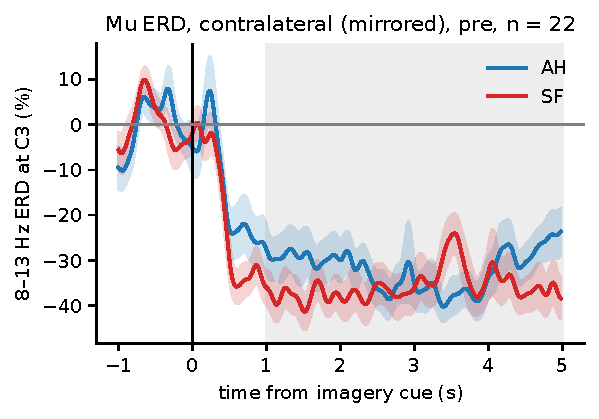
\includegraphics[width=0.9\linewidth]{eda_erd_timecourse.pdf}
  \caption{Mu-band (8--13\,Hz) ERD at C3, on the side opposite the affected hand (the
  channels of left-hemiplegic patients mirrored), pre-therapy session, \edaErdMuCThreeN{}
  patients. AH: imagined grasp of the affected hand; SF: imagined sixth finger. Bands are
  one standard error of the mean; the shaded span is the 4\,s window the decoders read. Look at
  how both movements fall by a similar amount and stay down: the two are hard to tell
  apart by this rhythm alone.}
  \label{fig:erd}
  \end{minipage}\hfill
  \begin{minipage}[t]{0.485\textwidth}
  \vspace{0pt}\centering

  % The 40 analysis channels seen from above, nose up, and the two groups of the channel ablation
% (src/sixthfinger/data/channels.py: CENTRAL_14, PARIETO_OCCIPITAL_5). Positions follow
% docs/figures/montage_40, spread a little where two discs would touch.
\begin{tikzpicture}[x=0.068mm, y=-0.068mm,
  ch/.style={circle, draw=black!70, line width=0.5pt, minimum size=5.9mm, inner sep=0pt,
    font=\fontsize{6}{6.5}\selectfont, fill=black!6},
  central/.style={ch, fill=rblue, text=white, draw=rblue!70!black},
  posterior/.style={ch, fill=rorange, draw=rorange!70!black}]
  \draw[line width=0.8pt] (541,568) circle (430);
  \draw[line width=0.8pt] (493,140) -- (541,82) -- (589,140);
  \draw[line width=0.8pt] (111,508) -- (82,525) -- (82,612) -- (111,630);
  \draw[line width=0.8pt] (971,508) -- (1000,525) -- (1000,612) -- (971,630);
  \foreach \n/\x/\y in {AF3/398/242, AF4/689/245, F5/247/349, F3/347/362, F1/446/372,
      Fz/541/373, F2/642/369, F4/740/358, F6/840/349, FC5/208/486, FC3/325/486, FC1/436/487,
      FCz/541/487, FC2/650/485, FC4/761/484, FC6/875/484, P5/300/838, P3/388/790,
      Pz/541/770, P4/698/788, P6/785/836}
    \node[ch] at (\x,\y) {\n};
  \foreach \n/\x/\y in {C5/215/623, C3/329/604, C1/438/595, Cz/541/592, C2/649/594,
      C4/758/602, C6/870/617, CP5/251/737, CP3/351/707, CP1/448/690, CPz/541/686,
      CP2/641/690, CP4/738/704, CP6/836/730}
    \node[central] at (\x,\y) {\n};
  \foreach \n/\x/\y in {PO5/372/918, PO3/452/874, POz/541/868, PO4/630/874, PO6/712/918}
    \node[posterior] at (\x,\y) {\n};
  \node[central, minimum size=4mm] (k1) at (80,1075) {};
  \node[anchor=west, font=\footnotesize, align=left] at (115,1075) {central 14};
  \node[posterior, minimum size=4mm] (k2) at (80,1140) {};
  \node[anchor=west, font=\footnotesize, align=left] at (115,1140) {parieto-occipital 5};
  \node[ch, minimum size=4mm] (k3) at (620,1075) {};
  \node[anchor=west, font=\footnotesize, align=left] at (655,1075) {other 21};
\end{tikzpicture}

  \caption{The 40 analysis channels seen from above, nose at the top, and the two groups of
  the channel ablation: 14 central channels over the motor strip (blue) and five
  parieto-occipital channels over the visual cortex (orange). The first should carry motor
  imagery; the second would carry a response to the picture shown during imagery.}
  \label{fig:channels}
  \end{minipage}
\end{figure}

\subsection{Tasks and calibration scenarios}
\label{sec:scenarios}
We studied three decoding tasks: the three-class problem of rest, hand and sixth finger
(chance is one third); sixth finger against rest, which detects the new command; and hand
against sixth finger, the contrast the dataset paper reports. Calibration was simulated on
the existing recordings (Fig.~\ref{fig:calib}). For every target patient, $k$ trials per
imagery class were sampled from runs 1--2 along with the rest windows before them, and the
resulting decoder was scored on runs 3--4 of that session. We used $k \in \{0, 1, 2, 3, 5, 10, \text{all}\}$, sampling each budget ten times (five times
for the networks) with draws shared by all methods, plus one chronological draw. Calibration time
is quoted at the nominal 14\,s per trial of the article, so one trial per movement costs
\rqTwoMinutesKOne\,min and the full pool \rqTwoMinutesKAll\,min; measured from the recordings
these become \rqTwoMinutesRecordedKOne{} and \rqTwoMinutesRecordedKAll\,min.

The calibration was run under two scenarios. A \emph{new user} (S1) records $k$ hand trials
and $k$ sixth-finger trials. For a \emph{new command} (S2) the hand trials of runs 1--2 are
already on file and only $k$ sixth-finger trials are new, so the three-class decoders train on
all hand trials, the $k$ new ones and the matching rest windows. By the plan, though, the S2
decoders of sixth finger against rest see only the new trials and their rest windows, never a
hand trial; on that task S1 and S2 thus differ only in the random draws, and neither extends a
hand decoder. That question is left to the own-hand control below.

\begin{figure}[!t]
  \centering
  \scalebox{0.85}{% Simulated calibration: the paper's protocol drawing with the budgets of the study.
\begin{tikzpicture}[x=13mm, y=8mm, font=\small,
  box/.style={draw, rounded corners=3pt, align=center, minimum height=11mm, line width=0.7pt},
  flow/.style={-{Stealth[length=2.2mm]}, line width=0.8pt, draw=black!75},
  dflow/.style={-{Stealth[length=2.2mm]}, line width=0.8pt, dashed, draw=rgrey},
  lbl/.style={font=\footnotesize, text=black!70}]
  \node[font=\small\bfseries, anchor=west] at (-0.1,3.1) {Target patient, one session};
  \foreach \r/\c/\t in {0/rblue/run 1, 1/rblue/run 2, 2/rred/run 3, 3/rred/run 4} {
    \draw[fill=\c!15, draw=\c] (\r*2,1.6) rectangle (\r*2+1.8,2.6);
    \node[font=\footnotesize] at (\r*2+0.9,2.1) {\t};
  }
  \draw[decorate, decoration={brace, amplitude=4pt, mirror}] (0,1.5) -- (3.8,1.5)
    node[midway, below=5pt, font=\footnotesize, align=center] (pool)
    {calibration pool: $k$ trials per class\\(ten random draws and one chronological)};
  \draw[decorate, decoration={brace, amplitude=4pt, mirror}] (4,1.5) -- (7.8,1.5)
    node[midway, below=5pt, font=\footnotesize, align=center] (test)
    {test runs: never used for fitting,\\alignment or selection};
  \node[box, draw=rblue, fill=rblue!8, minimum width=30mm] (srcp) at (-2.5,-1.7)
    {other patients\\\footnotesize source windows};
  \node[box, draw=rgreen, fill=rgreen!10, minimum width=36mm] (train) at (1.9,-1.7)
    {train the decoder\\\footnotesize from scratch: drawn trials only};
  \node[box, minimum width=30mm] (eval) at (5.9,-1.7) {score\\\footnotesize balanced accuracy};
  \draw[flow] (pool.south) -- (train.north);
  \draw[dflow] (srcp) -- node[lbl, above] {transfer} (train);
  \draw[flow] (train) -- node[lbl, above] {decoder} (eval);
  \draw[flow] (test.south) -- (eval.north);
\end{tikzpicture}
}
  \caption{Simulated calibration for one target patient and one session. The decoder learns
  from $k$ trials per class drawn from runs 1--2 and is scored on runs 3--4, which are never
  used for fitting, alignment or selection. A decoder from scratch sees only the drawn
  trials; a transfer decoder also sees every window of the other patients, never the
  target's linked partner. S1, new user: $k$ hand and $k$ sixth-finger trials with their rest
  windows; S2, new command: every hand trial of runs 1--2 and $k$ sixth-finger trials.}
  \label{fig:calib}
\end{figure}

\subsection{Research questions and hypotheses}
\label{sec:hyp}
Six confirmatory hypotheses and one exploratory hypothesis were fixed before the main study.
\begin{itemize}
  \item \textbf{H1} (RQ1): for hand against sixth finger, CSP+LDA scores higher with its
        filters fitted on every trial ahead of cross-validation, as the dataset's script does,
        than with all fitting confined to the training folds. \textbf{H1b}: identical code
        inflates accuracy in the same way on two healthy datasets.
  \item \textbf{H2a} (RQ2, S1, three classes): transfer and no transfer differ in the area
        under the learning curve over $k \in \{1, 2, 3, 5, 10\}$. \textbf{H2b}: the advantage
        of transfer is larger at $k = 5$ than with all trials.
  \item \textbf{H3} (RQ3, S2): the same area comparison, over $k \in \{1, 2, 3, 5\}$, for two
        co-primary outcomes: (a) sixth finger against rest and (b) three classes.
        \textbf{H3c}: at $k = 2$ and $k = 5$, transfer detects the sixth finger better than an
        \emph{own-hand decoder} trained without any sixth-finger trial.
  \item \textbf{H4} (RQ4, exploratory): when the recording is streamed continuously through
        the demonstrator's command gate, most sixth-finger imagery periods trigger the
        sixth-finger command.
\end{itemize}
The own-hand decoder is TS+LR fitted to the patient's hand and rest windows only, and any
output other than rest counts as the sixth finger. If it finds sixth-finger imagery just as
well, the sixth finger contributes nothing beyond a hand decoder.

\subsection{Metrics and statistics}
Decoders are scored by balanced accuracy, with each patient counted once, and differences are
given in percentage points. A calibration curve is condensed into one number, the normalised
area under the learning curve (ALC), adapted from the active learning
challenge~\cite{guyon2011}:
\begin{equation}
\mathrm{ALC} = \frac{1}{x_{\max} - x_{\min}} \int_{x_{\min}}^{x_{\max}}
\frac{\mathrm{BA}(x) - c}{1 - c}\, dx, \qquad x = \ln(1 + k),
\label{eq:alc}
\end{equation}
in which $\mathrm{BA}$ denotes balanced accuracy and $c$ chance, integrated by the trapezoid
rule across the budgets a test covers. A curve at chance scores 0 and a perfect one 1. We also
give $k^*$, the first budget at which a patient attains 60 or 70\,\%. Paired comparisons rely
on the Wilcoxon signed-rank test, with the rank-biserial correlation $r$ as effect size and
95\,\% confidence intervals (CIs) from 10\,000 bootstrap resamples of patients. The plan made
H1, H1b, H2b and H3c one-sided and H2a and H3 two-sided; $W$ denotes the positive-rank sum in
one-sided tests and the smaller of the two rank sums in two-sided ones, and Holm's correction
is applied inside each pre-registered family.

The outcome of every test was assigned to one of four categories defined in advance. A test is
\emph{supported} if its rule is met; \emph{contrary}, an option only for two-sided tests, if
the effect is significant the other way; \emph{partial} if a two-part test meets one part; and
\emph{inconclusive} otherwise, a verdict never taken to mean that no effect exists. A
one-sided test with its effect in the wrong direction is accordingly inconclusive. As robustness checks, the stroke tests were rerun on the post-therapy session (also with
sub-21 and sub-22 merged into a single value) and with the development patients removed, and
the calibration tests under the chronological draw.

\subsection{Pre-registration, deviations and prior knowledge}
\label{sec:prereg}
The analysis plan was frozen in the project's git repository with the tag \texttt{prereg-v1}
on a commit of 3 October 2026; the tag was added on 8 October. By then no decoder had been
fitted to any patient except the two development patients, leaving aside a single smoke test
of transfer. Both dates come from git itself, and no independent registry holds the plan. The
plan and its log of \nDeviations{} dated deviations can be obtained from the authors. Most log
entries settle a rule before any calibration result existed. Ahead of the confirmatory
results the networks were retrained, because they had been dropping the final, incomplete
batch of every epoch. Afterwards, the electrode-count study was abandoned, a sanity check
built on a mistaken premise was logged as failed, and the post hoc analyses were added, each
follow-up fixed in a settings file before it ran.

Some knowledge preceded the freeze: we had inspected labelled spectra and ERD maps for all
patients and sessions, and the development patients had already revealed the direction of
H1. Before the calibration study, the benchmark had also shown the full-pool accuracy without
transfer, which enters H2b, and the accuracy of the pre-trained EEGNet without calibration.
Exploratory tests carry no correction, apart from the planned Holm adjustment across budgets
for mirroring, and none of them alters a confirmatory category.
